%%%%%%%%%%%%%%%%%%%%%%%%%%%%%%%%%%%%%%%%%%%%%%%%%%%%%%%%%%%%%%%%%%%%%%%
%% Related Work
\section{Stand der Technik}
\label{sec:relatedwork}

In diesem Kapitel werden auf das Thema bezogene Forschungen vorgestellt und untersucht. Da es zu der genauen Thematik kaum Forschungen gibt, werden vor allem Teilaspekte der Arbeit aufgezeigt. Dazu gehört die Definition und Entwicklung von Multi-Robot-Systemen. In dieser werden die Kategorisierung von Multi-Robot-Systemen und Frameworks, sowie Architekturen, für die selbigen vorgestellt. Danach liegt der Blick unter anderem auf der Arbeit von Mathias Broxvall, in dieser wird die Einbindung eines Roboters in eine intelligente Umgebung untersucht. Darauf folgt ein Einblick in die Thematik des Greifens, sowie der Übergabe zwischen verschiedenen Teilnehmern.

%%%%%%%%%%%%%%%%%%%%%%%%%%%%%%%%%%%%%%%%%%%%%%%%%%%%%%%%%%%%%%%%%%%%%%%
%% Related Work
\subsection{Multi-robot system - Konzepte zur Verwaltung mehrerer Roboter}
\label{sec:relatedwork-multirobots}
    
Die Verwendung mehrerer individueller Roboter ist Forschungsthema seit 1986 und ist ein weit gestecktes Feld. Frühere Themen sind zelluläre Roboter, Motion Planning, Schwarmrobotik und Architekturen. Nach dem neuen Robotik Paradigma der behavior-based Kontrolle orientieren sich viele Forschungen an der Biologie und versuchen Abbildungen der sozialen Strukturen von Insekten und anderen Schwarmtieren zu nutzen.\cite{parker2003current} Dabei wurden zum Beispiel die Schwarmbildung (siehe \cite{hayes2002self}), die Futtersuche (\cite{balch1999impact}) und die Spurverfolgung (\cite{vaughan2000whistling}) betrachtet. Viele Probleme von Multi-Robot Systemen (MRS) haben oft einen Bezug zu Problemen aus anderen Forschungsgebieten und können durch die Anzahl an Robotern meist robuster und schneller gelöst werden. Weitere große Forschungsbereiche sind die verteilte künstliche Intelligenz und der Multi-Agent Ansatz. Beide befassen sich mit der Kooperation zwischen Systemen. Erste Ergebnisse dieser Bereiche wurden mit einer Prioritätsordnung der Subtasks erreicht\cite{durfee1987coherent}. Spätere Arbeiten betrachteten das Gruppieren von Systemen, die Aufgaben miteinander bearbeiteten \cite{shehory1998methods} und \cite{lau2003task}. Diese Gruppen, auch Koalitionen genannt, lösen Aufgaben, die nicht an einen einzelnen Roboter gestellt werden können. Die Arbeit \cite{vig2005issues} überführte dann die bekannten Lösungen der Koalitionen in die Probleme der MRS. Weitere Themen aus dem Bereich Multi-Agent, Team-Work (\cite{pynadath2003automated}), Potenzial-Management (\cite{timm2003ontology}) und Normen(\cite{boella2002norms}), wurden für die Koordinierung von MRS angewandt \citep{lundh2006plan}.

\subsubsection{Klassifizierung der Koordinierung}
Die Koordinierung von Robotern beschreibt die Organisation von Bewegungen, welche die Roboter zusammen ausführen sollen. Potenzielle Probleme sind dabei die Fragestellungen wie die Koordination organisiert werden soll, wer organisieren soll oder wie viel Koordination nötig ist um eine Aufgabe zu erledigen.

Bei den Organisationsmöglichkeiten unterscheidet man zwischen zentralisiert und verteilt. In einem stark verteilten System sind die einzelnen Roboter unabhängig und selbstständig. Entscheidungen werden meistens zwischen den Systemen ausgehandelt. Diese Variante ist gegenüber einem zentralen System robuster, da kein Single-Point-of-Failure auftritt. Dafür ist es meist komplexer eine optimale Lösung für ein Problem zu finden. Außerdem ist der Kommunikationsaufwand wesentlich höher. In einem stark zentralisiertem System übernimmt ein System die Führung und alle Entscheidungen. Das ganze kann dann als ein Robotersystem mit ferngesteuerten Sensoren und Aktoren abgebildet werden. Nachteilig ist hier der beschriebene Single-Point-of-Failure: Fällt das zentrale System aus, kann das ganze System nicht mehr arbeiten. Außerdem sind solche Systeme meist langsamer, da die ganzen Informationen erst auf einer Recheneinheit zusammengefasst werden müssen und anschließend dort ausgewertet werden. Dadurch können aber auch einfacher optimierte Lösungen gefunden werden \citep{lundh2006plan}. Weitere Informationen finden sich in den Arbeiten \cite{farinelli2004multirobot} und \cite{dias2003comparative}. 

Ein weiterer Aspekt der Koordinierung von MRS ist der benötigte Grad an Koordinierung. Dabei wird in der Literatur zwischen den Begriffen der engen (\textit{tight}), beziehungsweise eng-gekoppelt oder starken, Koordinierung und der losen (\textit{loosly}), lose-gekoppelt oder schwache, Koordinierung unterschieden. In der Arbeit \cite{farinelli2004multirobot} ist die starke Koordinierung als eine Koordinierung beschrieben, die auf einem Koordinationsprotokoll aufbaut. Ein Koordinationsprotokoll beschreibt eine Menge an Regeln die spezifizieren wie Roboter miteinander interagieren. Eine schwache Koordinierung baut nicht auf einem solchen Protokoll auf. Die Begriffe eng (eng-gekoppelt) und lose (lose-gekoppelt) definieren die Quantität der Koordinierung. Ein eng-gekoppeltes MRS benötigt viel Koordinierung, ein loses MRS eher wenig. Da die Begriffe viel und wenig ungenau und schwer zu definieren sind, existieren in der Literatur verschiedene Definitionen. Die Arbeit \cite{kalra2004hoplites} unterteilt die Koordinierung in \textit{loosly}, \textit{moderately} und \textit{tightly} anhand der Zerlegung der Aufgaben (Tasks) in Unteraufgaben (Subtasks). Bei eine losen Koppelung können alle Tasks in Subtasks zerlegt werden, die von einem Roboter ausgeführt werden können. Mäßige Kopplungen begrenzen die Koordination auf zeitlich abhängige Subtasks. Dabei beschränkt sich die Koordination nur auf den Startzeitpunkt ($t_0$) eines Subtasks. Die Ausführung des Tasks wird nicht koordiniert. Eine enge Kopplung erfordert eine permanente Koordination und Tasks können nicht in Subtasks zerlegt werden, die von einem Roboter abgearbeitet werden \citep{lundh2006plan}.

Eine weitere Klassifizierung der Literatur bezieht sich auf die Tasks. In der Definition von \cite{gerkey2004formal} wird zwischen \textit{single-robot} tasks (SR) und \textit{multir-robot} tasks (MR) unterschieden. SR benötigen genau einen Roboter für die Ausführung, zum Beispiel eine Bewegung an eine gewünschte Position. MR können mehrere Roboter benötigen. Außerdem werden Roboter eingegliedert.\textit{ Multi-Task} (MT) Roboter können gleichzeitig mehrere Tasks ausführen, \textit{Single-Task} Roboter führen immer nur Tasks nacheinander aus \citep{lundh2006plan}. 

\subsubsection{Probleme der Koordinierung}
Bei lose-gekoppelten MRS ist das Hauptproblem die Zuweisung der Tasks, da jeder Task ein SR ist. Dieses Problem wird als \textit{Task allocation} bezeichnet. Darauf baut das Problem der Rollenzuweisung auf, wenn im MRS mit einem Rollensystem gearbeitet wird. Task Allocation beschreibt wie eine Anzahl von Tasks auf eine Anzahl von Systemen verteilt wird. Die einfachste Aufteilung wurde schon 1960 in \cite{gale1989theory} beschrieben und seitdem in zahlreichen Arbeiten untersucht: Ein Task kann nur einem Agenten zugewiesen werden und jedem Agenten kann nur eine Task zur Zeit abarbeiten.

Ein bekannter Lösungsansatz ist das ALLIANCE-System von Lynne E. Parker aus dem Jahr 1998 \cite{parker1998alliance}. Dieser Algorithmus nutzt vier einfache Schritte zur Vergabe der Tasks. In einer Pärchen-Liste von Task-Agent sind alle möglichen Kombinationen im MRS gespeichert und werden nach der Nützlichkeit bewertet. (1) Finde das am besten bewertete Pärchen (2) weise die Task dem Agenten zu (3) entferne das Pärchen aus der Liste (4) ist die Liste nicht leer beginne mit (1), ansonsten terminiere. Der Vorteil von ALLIANCE liegt nicht in der Zuweisung, sondern in der Neuzuweisung. Dazu werden zwei Aspekte der Verhaltenssteuerung genutzt: Ungeduld (\textit{impatience}) und Fügung (\textit{acquiescence}). Ungeduld ermöglicht es,dass ein Agent eine Task eines anderen Agenten übernimmt. Wenn Roboter A die Eindruck bekommt, dass Roboter B die Task nicht lösen kann, wird er ungeduldig und übernimmt die Aufgabe. Die Fügung funktioniert ähnlich, nur das Roboter A feststellt, dass er selbst die Task nicht oder nicht gut genug lösen kann und diese an Roboter B abgibt. Weitere Forschungen gibt es unter anderem bei \cite{werger2000broadcast}.

Ein weiterer bekannter Ansatz für das Problem ist das \textit{Contract Net Protocol} (CNP) von Davis und Smith aus dem Jahr 1983. \cite{davis2003negotiation}. Das CNP beruht auf einem Auktionshausprinzip. Tasks werden von einem Dealer als Broadcast angeboten. Agenten im MRS haben die Möglichkeit privat auf die Tasks zu bieten. Dabei werden meist Ergebnisse des auszuführenden Task geboten. Diese Ergebnisse können unter anderem Energie- und Zeitkosten beinhalten. Der Dealer entscheidet wer den Zuschlag bekommt. Er kann auf Grund des Gebotes den bestmöglichen Agenten für die Task bestimmen. Die Auswahl kann dynamisch, je nach Priorität (zum Beispiel Zeit vor Energiekosten), ausgewählt werden. Varianten die auf CNP basieren sind GOFER \cite{caloud1990indoor}, M+ \cite{botelho1999m+}, TraderBots\cite{dias2000market} und Sold! \cite{gerkey2002sold}.

Bei Rollenbasierten Ansätzen werden einzelnen Agenten Rollen zugewiesen und dadurch in ihrer Funktionalität beschränkt. Agenten mit den gleichen Rollen haben die gleichen Funktionalitäten. Ansätze dafür finden sich in den Arbeiten \cite{frias2005exploring}, \cite{vail2003multi} und \cite{stone1999task}.

Bei eng-gekoppelten MRS ist die primitive Zerlegung wie bei losen Systemen nicht möglich. Dadurch fällt die Koordinierung nicht nur in der Startphase an, sondern auch während des Prozesses. Zentrale Probleme sind nicht nur der Ausführer, sondern die Frage nach der Ausführung, also wie eine Task erledigt wird. Ein möglicher Anwendungsfall ist die Arbeit von \cite{saffiotti2000multi}. Bei diesem Ansatz arbeiten Roboter in einer Formation. Jeder Roboter besitzt dabei zwei Vorsätze, das Team-Ziel und das Individualziel. Das Team-Ziel ist das übergeordnete Gemeinschaftsziel, zum Beispiel das Tragen eines Objektes. Das Individualziel sind Roboter-eigene Interessen, zum Beispiel die Kollisionsvermeidung. Typische Lösungsansätze für solche Anwendungen ist das Führer-Folger Prinzip, bei dem ein Führer bestimmt wird, dieser übernimmt Entscheidungen, die Folger folgen dem Führer. Dies ist bei komplexeren Anwendungen jedoch nicht ausreichend, sodass eine Planung notwendig wird. Dabei treten die beiden zentralen Fragen auf:\textbf{ Wer macht was?} und\textbf{ Wie wird es gemacht?}.

Das Robotik Institute der Carnegie Mellon University hat eine Forschungsgruppe, die sich mit der Frage nach dem \textit{wer} beschäftigt. Dabei werden drei Ansätze verfolgt. Die erste beschäftigt sich mit der Aufgabenverteilung bei komplexen Tasks, die zweite mit der Aufgabenverwaltung bei eng-gekoppelten MRS und die dritte mit Architekturen für enge MRS. Als Grundlagen dient den dreien die schon erwähnte Arbeit von Dias und Stentz, den TraderBots\cite{dias2000market} die auf dem CNP aufbauen. Die Arbeit \cite{zlot2005complex} befasst sich mit der Aufgabenverteilung bei komplexen Tasks. Dabei werden komplexe Tasks als Aufgaben mit mehreren Lösungswegen definiert. Die Erstellung eines Plans für eine komplexe Task liegt meist in \textit{NP-hard}. Im Gegensatz dazu stehen die einfachen (simple) Tasks, die einfach vorwärts gerichtet sind. Ähnlich dem Auktionsverfahren wurde so ein Auktionsansatz für komplexe Tasks entwickelt. Anstatt eine primitive Task anzubieten werden Taskbäume angeboten. Dabei entspricht die Wurzel dem abstrakten komplexen Task, die Knoten den komplexen Subtasks, die Blätter den primitiven Subtasks und die Kanten dem Koordinationsaufwand. Die einzelnen Agenten können nun auf die Blätter bieten. Die zweite Forschungsrichtung befasst sich mit einem Marktansatz für eng-gekoppelte Systeme und wird in den Arbeiten \cite{kalra2004hoplites} und \cite{kalra2005hoplites} behandelt. Das Konzept trägt den Namen Hoplites und lässt sich aus dem antiken Griechenland herleiten. Dort waren die Hopliten eine der besten Infanterieeinheiten und auf komplexe Manöver spezialisiert. Bei diesem Framework werden Agenten rückwirkend bewertet. Die Bewertung erfolgt nach Beendigung eines Task und gibt an wie sehr dieser Agent dem Gemeinschaftsziel gedient hat. Des weiteren nutzt das Framework aktive und passive Koordinierung ein. Passive Koordinierung wird für simple Tasks eingesetzt und solange genutzt, bis die aktive Koordinierung bessere Vorhersagen bietet. Das Framework selbst hat keinen Planer für komplexe Aufgaben, sondern entscheidet nur, wann welcher Planer eingesetzt werden soll. Der dritte Aspekt behandelt Architekturen für eng-gekoppelte MRS und heterogenen Roboter. Die Arbeiten \cite{simmons2001first} und \cite{simmons2002layered} zeigen eine drei Schichten Architektur. Diese Schichten (Planungs-, Ausführungs- und Verhaltensschicht) können innerhalb eines Roboters miteinander kommunizieren. Außerdem können die einzelnen Schichten auch Roboter übergreifend kommunizieren. Also Planungsschicht von Roboter A mit Planungsschicht von Roboter B, aber nicht mit Ausführungsschicht von Roboter B \citep{lundh2006plan}.

%\begin{figure}[H]
%	\centering
%	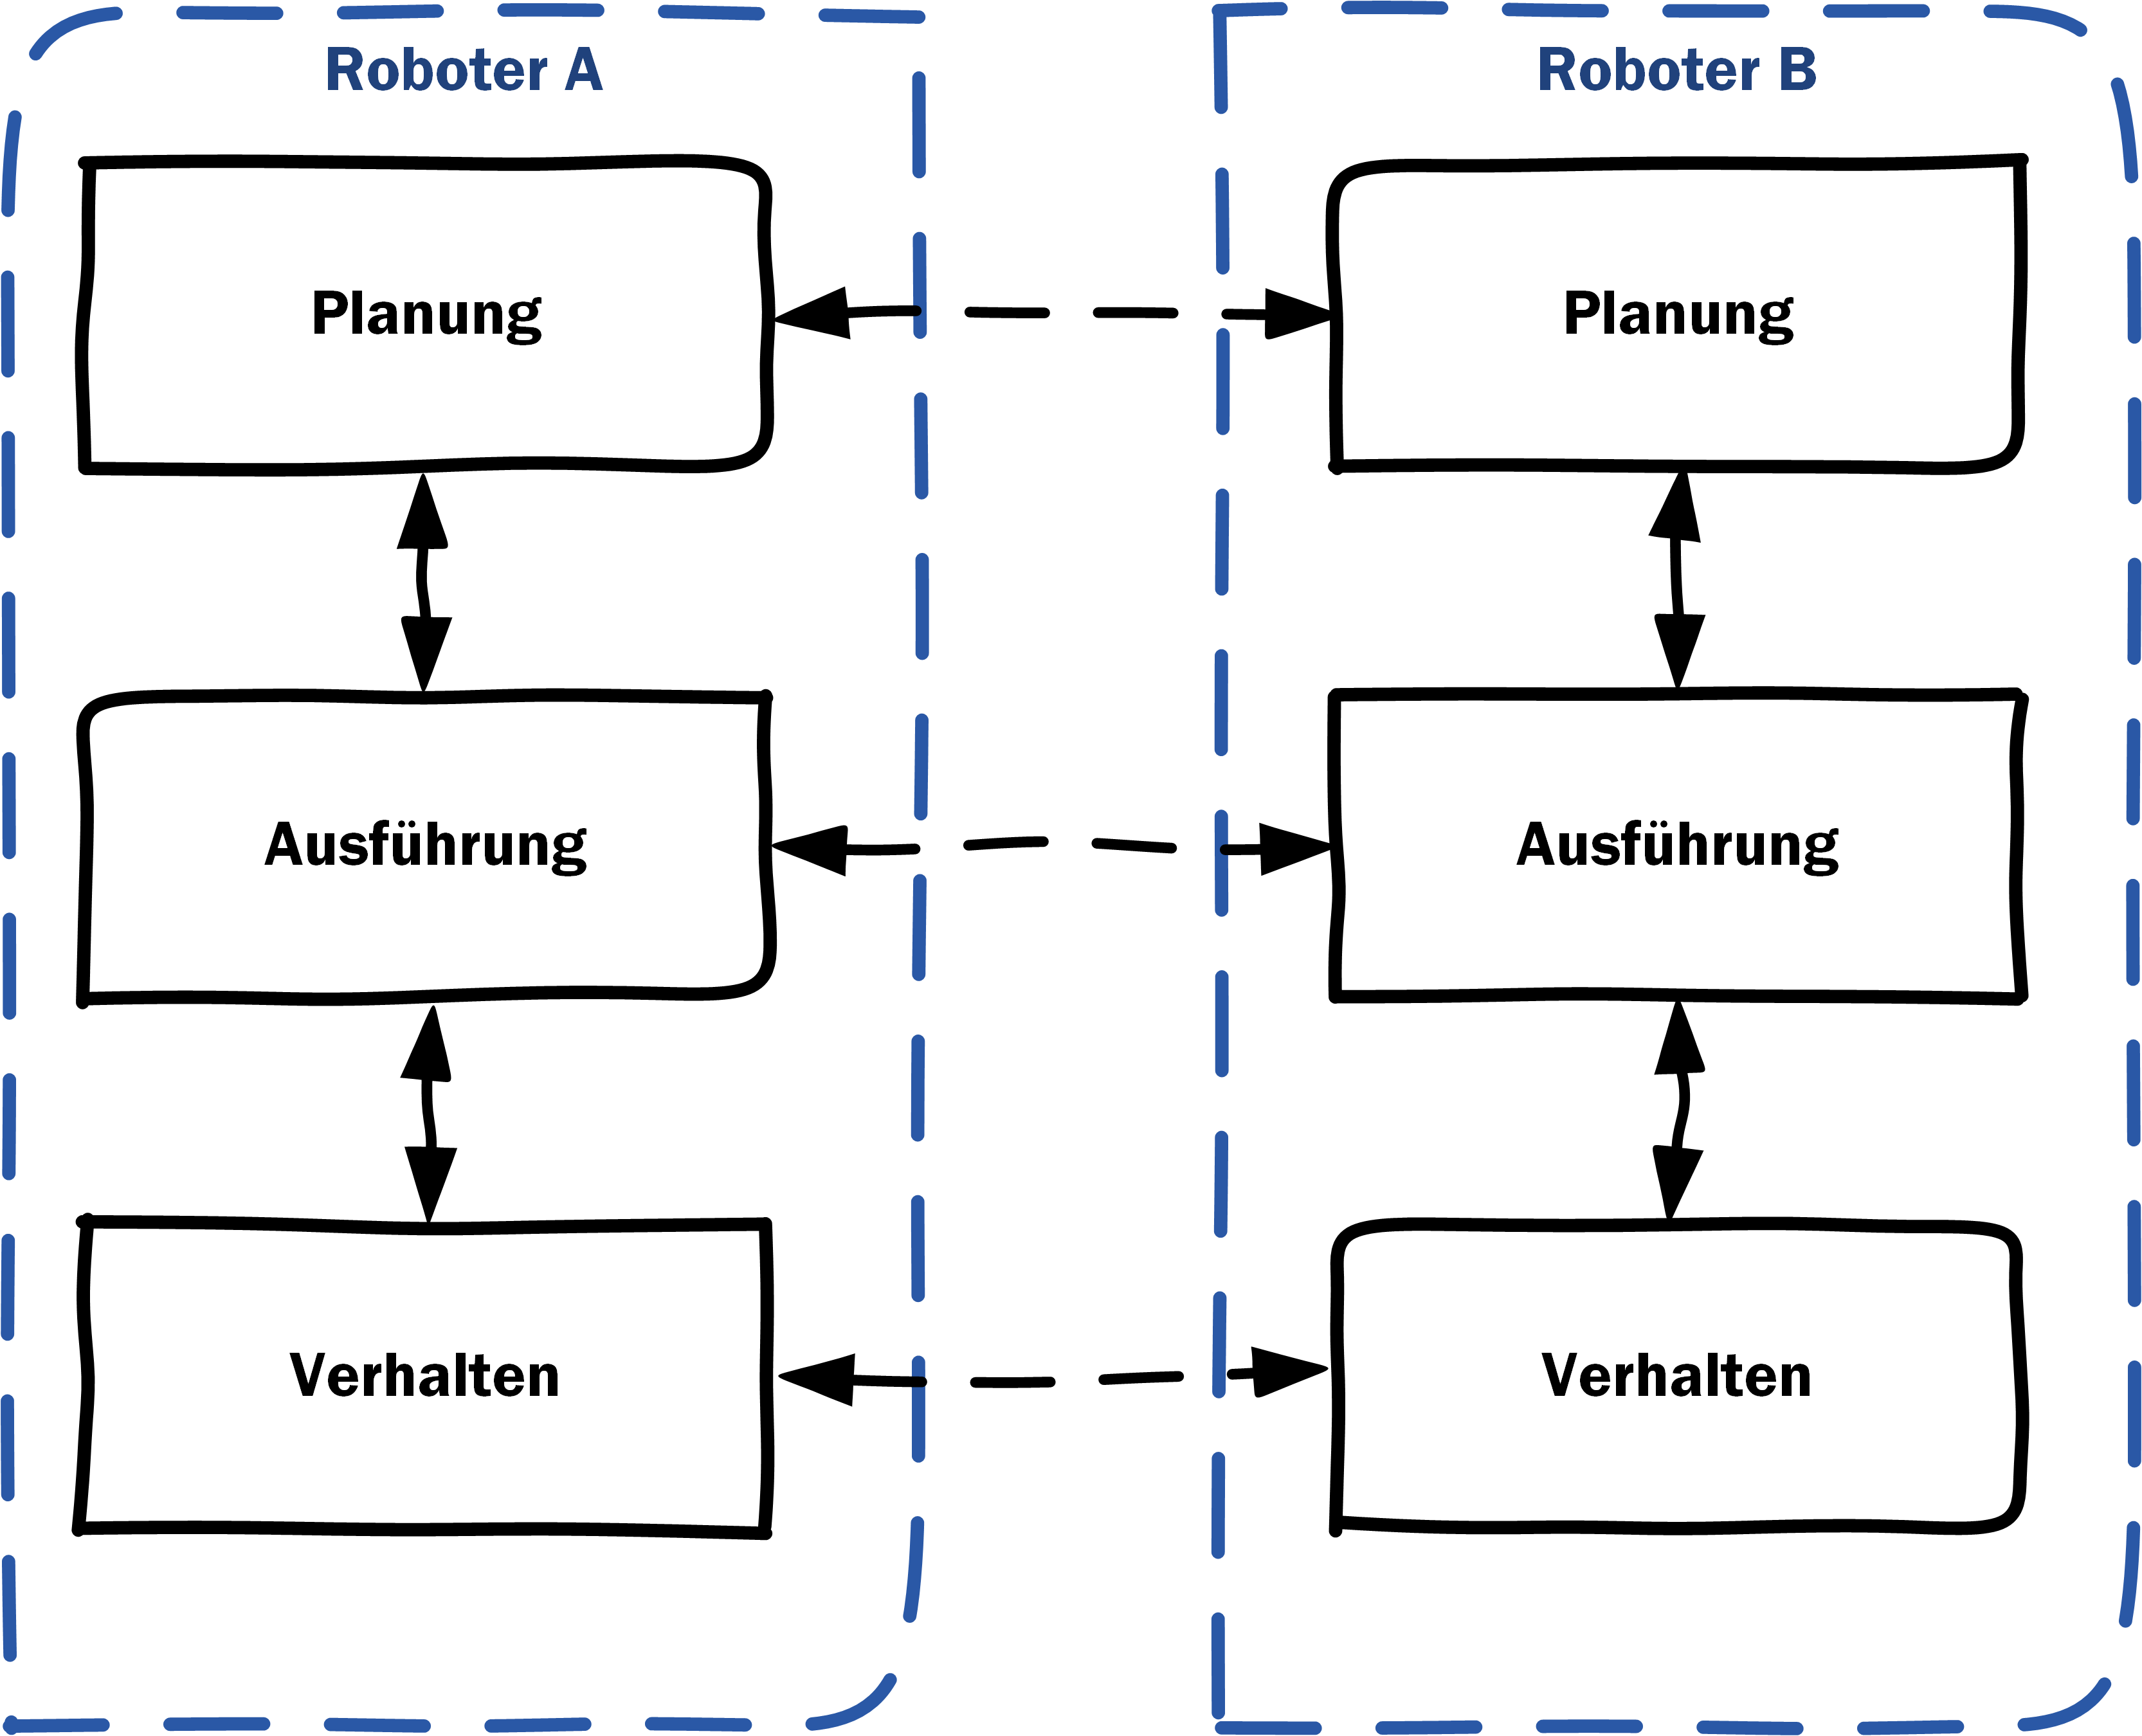
\includegraphics[scale=0.6]{fig/layer}   
%	\caption[Three-Layer Architektur]{Drei Schichten Architektur zur Koordinierung von eng-gekoppelten Systemen. Übernommen aus: \cite{simmons2002layered}}
%	\label{fig:sota-layer}
%\end{figure}

Die schon zitierte Lynne E. Parker leitet die Forschungsgruppe des \textit{Distributed Intelligence Laboratory} an der University of Tennessee. Die zentralen Forschungen der Gruppe befassen sich mit der automatischen Koordination von Roboterteams. 2003 und 2004 präsentierte Parker zwei Arbeiten \cite{parker2003effect} und \cite{parker2004tightly} in denen Netzwerke von über 70 Robotern eng koordiniert wurden. Dabei wurde zwischen sensorarmen und -reichen Robotern unterschieden. Für die enge Kopplung wurde dabei ein Führer-Folger Prinzip gewählt. Als Führer wurden die sensorreichen Roboter ausgewählt. In der Arbeit wurden zwei Tasks bearbeitet. Die erste wurde als Long-Distance-Navigation beschrieben, dabei übernimmt ein Führer die Kontrolle und berechnet einen Weg mit seinen Sensoren. Die sensorarmen Roboter folgen dem Führer. Am Ziel angekommen bauen alle Roboter ein gemeinsames Sensornetzwerk auf und überwachen den Zielraum. Die Roboter innerhalb des Sensornetzwerkes versorgen sich dabei automatisch mit den benötigten Informationen. Die Konfiguration für dieses MRS ist jedoch statisch durch die Entwickler vorgegeben. In der anschließenden Veröffentlichung \cite{parker2005enabling} stellte die Forschungsgruppe \textit{ASyMTRe} (Automated Synthesis of Multi-robot Task solutions through software Reconfiguration) vor. Dieses Konzept, beruhend auf der Schemen Theorie aus \cite{arkin1987motor}, ermöglicht einem MRS eng-gekoppelte Tasks durch Informationsaustausch zu lösen. Dazu werden verschiedene Schemen so miteinander verbunden, dass die Informationen von den Umweltsensoren zu den Motor-Schemen gelangen. ASyMTRe nutzt dazu einen Algorithmus, der alle Informationen für den am wenigsten fähigen Roboter sammelt und diese anschließend an alle verteilt. Anschließend wird der Roboter als Führer ermittelt, der den größten Informationsgehalt bei kleinster Sensorik hat \citep{lundh2006plan} .

\subsubsection{Zusammenfassung}
Dieses Kapitel zeigte Arbeiten und Konzepte rund um das Thema Multi-Robot Systeme auf. In dieser Zusammenfassung sollen die benötigten Informationen für diese Arbeit extrahiert und Entscheidungen für die eigene Entwicklung getroffen werden. In diesem Kapitel wurden zunächst die Begriffe Koordination und Konfiguration durch verschiedene Arbeiten definiert. Außerdem wurden die Begriffe verteilte und zentrale, starke und schwache, sowie enge und lose Koordination erläutert. In den Arbeiten stellte sich heraus, dass zentrale Steuerungen durch einen Single-Point-of-Failure durch Störungen stärker betroffen sind als verteilte Koordination. Diese wiederum benötigt einen größeren Aufwand der Algorithmen und der Konfiguration. Daraus folgt für diese Arbeit, dass ein erster Entwurf eine zentrale Koordinierung haben wird, da der Aufwand beschränkt ist. Jedoch soll eine Schnittstelle für eine verteilte Koordinierung vorgesehen werden. Aus der Literatur ergab sich, dass starke Koordination auf einem Koordinationsprotokoll aufbauen und schwache auf dynamischen Algorithmen, die beteiligte Robotersysteme auswählt. Da in dieser Arbeit nur zwei Roboter verwendet werden und diese zwangsweise miteinander arbeiten müssen ist die Auslegung eines dynamischen Zuweisungsmodell überflüssig, soll aber auch in Form von Schnittstellen für weitere Aufgaben vorgesehen werden. Die Begriffe der eng- und lose-gekoppelten MRS wird durch verschiedene Definitionen unterschiedlich ausgelegt. Für diese Arbeit wird auf die Definition von \cite{kalra2004hoplites} zurückgegriffen. Da in dieser die Begriffe anhand der Zerlegung von Tasks definiert werden, kann die Kategorisierung für dieses System erst nach der Anforderungsanalyse geschehen. Auch die Eingliederung der Tasks in Single-Robot und Multi-Robot Tasks kann erst nach der Anforderungsanalyse erfolgen. Dies betrifft ebenfalls die Entscheidung für Single-Task oder Multi-Task Roboter. Auf ein Rollensystem soll zunächst verzichtet werden, da auch dies für dieses kleine System unnötiger Aufwand ist. Eine Erweiterung die für dieses System vorgesehen ist, beschreibt die Arbeit \cite{davis2003negotiation} mit dem CNP. Die Vergabe der Aufgaben mit Hilfe eines Auktionshauses kann in zukünftigen Entwicklungsschritten auch für komplexere, sogar eng-gekoppelte, MRS genutzt werden. Im folgenden Kapitel wird die Architektur PEIS vorgestellt, die neben Robotersystemen auch weitere Sensoren und Aktoren einschließt. Diese Architektur soll als Ausgangsarchitektur dienen.
%%%%%%%%%%%%%%%%%%%%%%%%%%%%%%%%%%%%%%%%%%%%%%%%%%%%%%%%%%%%%%%%%%%%%%%
%% Related Work
\subsection{Physically Embedded Intelligent Systems - PEIS}
\label{sec:relatedwork-peis}
    
    Andere beschäftigen sich grad mit \ldots



%%%%%%%%%%%%%%%%%%%%%%%%%%%%%%%%%%%%%%%%%%%%%%%%%%%%%%%%%%%%%%%%%%%%%%%
%% Related Work
\subsection{Grasping und Handover - Arbeiten zu Roboterarmen}
\label{sec:relatedwork-handover}
Dieses Kapitel befasst sich mit Arbeiten zu dem Thema Roboterarme. Zunächst wird das Greifen eines Gegenstandes, \textit{Grasping}, aufgezeigt. Dabei werden Arbeiten zum allgemeinen Greifen, zur Erkennung geeigneter Greifpositionen an Gegenständen und Kamera-unterstütztem Grasping aufgeführt. Im Anschluss wird die Thematik der Übergabe, dem zentralen Thema dieser Arbeit, aufgegriffen und Literatur zu Roboter-Mensch Übergaben betrachtet.

\subsubsection{Grasping - Greifen mit einem Roboterarm}
Als Ausgangsarbeit für dieses Thema bietet sich die Arbeit \cite{bicchi2000robotic} an. In dieser werden die Grundlagen des Greifens erläutert. Dabei wird zunächst die menschliche Hand und ihre Verwendungszwecke betrachtet. Der Mensch nutzt seine Hand zur Erkundung, zum Festhalten und zur Manipulation von Objekten. Das Erkunden von Objekten ist der eigene große Forschungsbereich \textit{Haptik} und kann bisher, auf Grund von fehlender Sensorik, in der Robotik nicht vollständig eingesetzt werden. Zwischen dem Festhalten, Fixieren und der Manipulation wird in der Arbeit unterschieden, sowie zwischen dem Manipulieren mit den Fingern und der Manipulation mit dem gesamten Arm. Dies liegt vor allem an den Anwendungs- und Forschungsbereichen. Während das Fixieren eines Objektes, beziehungsweise die Manipulation mit dem gesamten Arm, in der Industrie oft eingesetzt wird, ist die filigrane Arbeit mit den Fingern noch ein Thema der Forschung. Die ersten Arbeiten zu diesem Thema der Robotik gehen auf \cite{asada1979studies}  und \cite{mason1985robot} zurück. Neben dem Greifen mit den Fingern der Hand gibt es auch Griffe mit dem kompletten Arm, bezeichnet mit \textit{whole arm graps} \citep{townsend1988effect}, \citep{bicchi1994problem} und \textit{power grasps} (\citep{mirza1990force}) \citep{bicchi2000robotic}. 

Das Greifen unterliegt physischen Grenzen. Dabei wird der Griff, beziehungsweise das Halten, unter anderem durch den Kraftvektor und dem Haftkoeffizienten beeinflusst. Ein Griff wird durch $N$ Kontakte beschrieben. Dabei wird angenommen, dass alle Kontakte punktuell sind. Auch ein Kontakt auf einer Linie oder Oberfläche wird durch zwei oder mehr Punktkontakte abgebildet. Die Literatur unterscheidet diese Kontakte in reibungslose, reibungsbedingte oder weiche Punktkontakte \citep{salisbury1983kinematic}. Ein reibungsloser Kontakt kann nur eine Kraft entlang der gemeinsamen Normalen erzeugen. Ein reibungsbedingter kann neben der normalen auch eine tangentiale Kraft und ein weicher Kontakt zusätzlich ein Drehmoment erzeugen. Die Kontaktart ist abhängig von den Oberflächeneigenschaften des Greifers und des Objektes. Bei einer gummiähnlichen Oberfläche des Greifers wird der Kontakt als weich modelliert. Haben Greifer und Objekt beide harte und raue Oberflächen wird ein reibungsbedingter Kontakt angenommen. Sind die Kontaktstellen auf Greifer und Objekt glatt und ist ein kleiner Reibungskoeffizient gegeben, gilt der Kontakt als reibungslos \citep{bicchi2000robotic}.


Neben dem Greifen selbst existiert auch die Problematik des Greifpunktes. Also der Stelle am Objekt, an welcher der Greifer ansetzt. Dazu existieren verschiedene Arbeiten. Die ersten zu diesem Thema waren die Arbeiten \cite{kamon1996learning}, \cite{coelho2001developing} und \cite{bowers2003manipulation}. In diesen werden mit Hilfe von Sensoren planare 2D-Objekte gegriffen. Ergebnisse mit 3D-Objekten erreichte die Arbeit \cite{saxena2008robotic}. Dabei werden zunächst mit maschinellem Lernen und gelabelten Testdatensätzen gute Griffpunkte für 3D-Objekte angelernt. Anschließend kann der Algorithmus unbekannte 3D-Objekte bewerten und die besten Griffpunkte finden. Diese Grundlagenforschung wird in der Arbeit \cite{maitin2010cloth} genutzt um an unbekannten 3D-Objekten aus Stoff Ecken zum Greifen und Zusammenlegen zu finden. In dieser werden vor allem Ansätze nach dem RANSAC-Verfahren gewählt, um bestimmte Strukturen gezielt zu finden. Für weitere Informationen lassen sich in der Literatur noch viele verschiedene Anwendungsfälle und Ansätze zum Greifen finden.

\subsubsection{Handover - Übergabe zwischen zwei Systemen}
Die Übergabe zwischen zwei Systemen ist eine häufige Interaktion im Alltag. Dieses betrifft oft die Manipulation eines Objektes. Die Arbeit \cite{huber2008human} beschäftigt sich mit der Übergabe zwischen Mensch und Roboter und beinhaltet zunächst eine Analyse einer Übergabe zwischen zwei Menschen. Dabei stellt sich folgende Aktionsreihenfolge für eine Übergabe heraus \citep{huber2008human}:

\begin{enumerate}
	\item Der Geber nimmt das Zielobjekt
	\item Der Geber bewegt die Hand Richtung Übergabeposition
	\item Der Nehmer bewegt die Hand Richtung Übergabeposition
	\item Transaktion
	\item Beide nehmen ihre Hände zurück
\end{enumerate}

Eigene Beobachtungen vom Mensch-Mensch Übergaben ergaben, dass diese Form der Übergabe nur eine Interaktionsart ist und als \textit{Geben} bezeichnet werden kann, da die Interaktion vom Geber ausgeht. Eine Alternative dazu stellt das \textit{Nehmen} dar, bei dem die Interaktion vom Nehmer ausgeht. Eine optimierte dritte Interaktionsart wäre eine synchrone Bewegung beider Akteure, bei der eine Verzögerung durch die Reaktionszeit des Interaktionspartners entfällt.

In der Robotik existieren mehrere Arten der Übergabe. Diese unterscheiden sich anhand des Interaktionspartners und des Anwendungsfeldes. 
In der Industrie, zum Beispiel dem Automobilbau, werden die Werkstücke nicht direkt zwischen den einzelnen Robotern übergeben, sondern befinden sich auf einem Förderband. Dieses fährt das Werksstuck auf eine definierte Position und die einzelnen Roboter führen ihren Arbeitsschritt aus. Anschließend wird das Werksstück zur nächsten Station gebracht. Eine weitere Art der Übergabe ist die Mensch-Roboter-Interaktion. Dieses Thema ist ein weitverbreitetes Thema mit vielen Aspekten. So beschäftigen sich die Arbeiten \cite{huber2008human} und \cite{shibata1995experimental} mit dem Timing-Verhalten, \cite{mainprice2010planning} und \cite{kulic2005safe} befassen sich mit der sicheren Planung von Übergabe-Interaktionen. Weitere Arbeiten (unter anderem \cite{prada2014implementation} und \cite{basiliapproach}) beschäftigen sich mit den Reaktionen auf menschliche Aktionen, wie Gesten (zum Beispiel: Handfläche nach oben geöffnet als Geste fürs Nehmen) und Veränderungen während der Übergabe.

In dieser Arbeit steht jedoch die Roboter-Roboter-Übergabe im Fokus. Dieses Thema ist in der Literatur nicht vorhanden oder wird nur als Randaspekt erwähnt.
